\documentclass[12pt]{book}

\usepackage[toc]{appendix} % para crear ambientes de apéndice
\usepackage{amsmath,amssymb, amsthm} % Para mejorar ecuaciones
\usepackage[utf8]{inputenc}
\usepackage[spanish]{babel} % Español
\usepackage[nice]{nicefrac}  % Para mejorar fracciones
\usepackage{graphicx} % Para insertar graficos
\usepackage{float} % Para manejar la ubicacion de graficos
\usepackage[colorlinks=true, allcolors=black]{hyperref} % Para hipervincular las referencias dentro del texto
\usepackage[Conny]{fncychap} % Capítulos

\usepackage{marginnote}% Paquete para notas al márgen
    \setlength{\marginparwidth}{4cm} % Ancho de la nota al margen
    \setlength{\marginparsep}{0.5cm} % Distancia mínima entre la nota y el texto principal
\usepackage{multirow,array}


\begin{document}

Apuntes del ramo de Economía Política con el profesor Landerretche. Podría contener errores y en caso de encontrarlos por favor notificarme al correo: joamartine@fen.uchile.cl

Última actualización: Julio 2024

\newpage

\setcounter{chapter}{3}

\chapter{Organización Industrial}

\subsection*{Introducción a la teoría de juegos}
La teoría de juegos es una manera de modelar distintos tipos de interacciones de competición, cooperación y otras. Modelar qué decisión y el por qué puede ser tan simple como complejo dependiendo de los factores que que consideremos relevantes. En este capítulo se trataran los juegos simultáneos en secuencia e iterados (también llamados repetidos). 

\section{Juegos simultaneos}

En juegos simultáneos los agentes toman decisiones al mismo tiempo, estas decisiones interactuan resultando en \textbf{pagos}. El pago a cada persona refleja un nivel de utilidad, por lo que cada agente buscará llegar a un resultado del juego (la combinación de acciones) que maximize su pago. 

Para dos agentes $A$ y $B$ cada uno toma la decisión $X$ o $Y$, la combinación de decisiones llevará a cierto nivel de pagos. Este escenario puede ser representado por una \textbf{matriz de pago}\marginnote{\textbf{Matriz de pago:} La matriz de pago es una representación de los pagos un juego simultáneo para un número definido de individuos y estrategias.}[-3cm] en el cuadro \ref{cuadro: matriz de pago genérica}.

\begin{table}[!htbp]
  
  \centering
  \caption{Matriz de pagos}
  \setlength{\extrarowheight}{2pt}
  \label{cuadro: matriz de pago genérica}
  \begin{tabular}{*{4}{c|}}
    \multicolumn{2}{c}{} & \multicolumn{2}{c}{$B$}\\\cline{3-4}
    \multicolumn{1}{c}{} &  & X  & Y \\\cline{2-4}
    \multirow{2}*{$A$}  & X & $(a,b)$ & $(c,d)$ \\\cline{2-4}
    & Y & $(e,f)$ & $(g,h)$ \\\cline{2-4} 
  \end{tabular}
\end{table}

Ejemplifiquemos cómo se lee la tabla. Si $A$ tomó la estrategia $X$ y $B$ toma la decisión $Y$ entonces los pagos correspondientes son $(c,d)$, donde $c$ es el pago para $A$ y $d$ el pago para $B$. De la misma manera si $A$ elije $Y$ y $B$ decide $Y$ la matriz de pagos será $(g,h)$. 

Hay un componente estratégico en la interacción de $A$ y $B$ pues los pagos que reciba cada uno dependerá de la decisión que tome el otro. Por ejemplo si $A$ sabe que $B$ decide $X$ entonces $A$ elegirá la estrategia que maximize sus pagos. Específicamente $A$ está decidiendo con respecto a los pagos en negrita en el cuadro \ref{cuadro: B decide X}.

\begin{table}[!htbp]
  \centering
  \caption{Matriz de pagos con $B$ decidiendo $X$} \label{cuadro: B decide X}
  \setlength{\extrarowheight}{2pt}
  \begin{tabular}{*{4}{c|}}
    \multicolumn{2}{c}{} & \multicolumn{2}{c}{$B$}\\\cline{3-4}
    \multicolumn{1}{c}{} &  & X  & Y \\\cline{2-4}
    \multirow{2}*{$A$}  & X & $(\textbf{a,b})$ & $(c,d)$ \\\cline{2-4}
    & Y & $(\textbf{e,f})$ & $(g,h)$ \\\cline{2-4}  
  \end{tabular}
\end{table}

La decisión que tome $A$ dependerá qué pago es mayor, $a$ ó $e$, si es $a$ entonces elije $X$ y caso contrario elije $Y$.

\subsection{Estrategias y resolución de juegos}

\subsection{Equilibrios de Nash y óptimos de pareto en juegos}

\subsection{Juegos canónicos}

\subsubsection*{Dilema del prisionero}

El dilema del prisionero describe la situación en que dos criminales sospechosos son detenidos y separados para un proceso de interrogación. Si uno de los dos delata al otro y su complice no, este último tendrá pena de cárcel y el delator quedará libre. En caso de que los dos se delaten entre sí, ambos son condenados a años de cárcel. Por útlimo si ninguna se delata entre sí, quedan libres o cumplen penas menores.

La matriz de pago específicamente se en el cuadro. A mayor pena menor es el pago. 

\begin{table}[!htbp]
    \centering
    \caption{El dilema del prisionero}
    \setlength{\extrarowheight}{2pt}
    \begin{tabular}{*{4}{c|}}
      \multicolumn{2}{c}{} & \multicolumn{2}{c}{Prisionero $B$}\\\cline{3-4}
      \multicolumn{1}{c}{} &  & Cooperar  & Delatar \\\cline{2-4}
      \multirow{2}*{Prisionero $A$}  & Cooperar & $(-2,-2)$ & $(-10,-1)$ \\\cline{2-4}
      & Delatar & $(-1,-10)$ & $(-6,-6)$ \\\cline{2-4}
    \end{tabular}
  \end{table}

Cada uno tiene una estrategia dominante en delatar al otro, el resultado es un equilibrio de Nash sub-óptimo en términos de Pareto. 

El juego describe como dos personas no cooperan incluso si ello va en contra del interés de las dos. 

\subsubsection*{Mano invisible}

Si se deja la autorregulación de los mercados, dado que los individuos persiguen su propio interés, se produce un equilibrio que es un óptimo de Pareto. Una matriz que lo representa puede ser.

El agente $A$ tendrá una estrategía dominante, la cual será la opuesto a la del otro agente $B$. Finalmente el equilibrio de Nash es eficiente paretianamente.

\begin{table}[!htbp]
    \centering
    \caption{La mano invisible}
    \setlength{\extrarowheight}{2pt}
    \begin{tabular}{*{4}{c|}}
      \multicolumn{2}{c}{} & \multicolumn{2}{c}{Agente $B$}\\\cline{3-4}
      \multicolumn{1}{c}{} &  & $X$  & $Y$ \\\cline{2-4}
      \multirow{2}*{Agente $A$}  & $X$ & $(0,10)$ & $(1,1)$ \\\cline{2-4}
      & $Y$ & $(11,11)$ & $(10,0)$ \\\cline{2-4}
    \end{tabular}
  \end{table}

%(Aquí se podría citar a Adam Smith)

\subsubsection*{Guerra de los sexos}

Una pareja heterosexual se encuentra incomunicada en medio de un festival de metal. El hombre es fan de Metallica y la mujer fan de Megadeth. 

\begin{table}[!htbp]
    \centering
    \caption{Guerra de los sexos}
    \setlength{\extrarowheight}{2pt}
    \begin{tabular}{*{4}{c|}}
      \multicolumn{2}{c}{} & \multicolumn{2}{c}{Mujer}\\\cline{3-4}
      \multicolumn{1}{c}{} &  & Metallica  & Megadeth \\\cline{2-4}
      \multirow{2}*{Hombre}  & Metallica & $(2,1)$ & $(1,1)$ \\\cline{2-4}
      & Megadeth & $(0,0)$ & $(1,2)$ \\\cline{2-4}
    \end{tabular}
  \end{table}

  Cada uno tiene estragia dominante por ir al concierto de su banda preferida idependiente de lo que haga el otro, hay dos equilibrios de Nash por lo tanto este juego tiene ser resuelto con estrategias mixtas.

\subsubsection*{La caza del venado}
Dos individuos van a cazar ya sea conejos o venados y deben escoger su presa sin conocer la elección del otro cazador. Para cazar el venado (un premio mayor) requieren de la ayuda del otro, mientras que un conejo puede ser cazado por cada uno. Por lo tanto, si cooperan cazando al venado podrán ambos obtener más beneficios y estár en un óptimo de Pareto.

\begin{table}[!htbp]
    \centering
    \caption{La caza del venado}
    \setlength{\extrarowheight}{2pt}
    \begin{tabular}{*{4}{c|}}
      \multicolumn{2}{c}{} & \multicolumn{2}{c}{Cazador $B$}\\\cline{3-4}
      \multicolumn{1}{c}{} &  & Venado  & Conejo \\\cline{2-4}
      \multirow{2}*{Cazador $A$}  & Venado & $(4,4)$ & $(0,3)$ \\\cline{2-4}
      & Conejo & $(3,0)$ & $(3,3)$ \\\cline{2-4}
    \end{tabular}
  \end{table}
En este caso no existen estrategias dominantes, lo que lleva a la existencia de dos equilibrios de Nash, cazar al venado juntos domina paretianamente a cazar conejos juntos. Lo anterior representa un problema de cooperación social y una dicotomía entre seguridad y cooperación. 
\subsubsection*{Chicken}

Se trata de un juego para determinar quien es el más valiente, dos personas se posicionan con sus autos en dos extremos y aceleran de manera que llegará un punto en que choquen entre si. El primero que doble para evitar el impacto es un gallina, dejando al ganador como valiente. Hay tres escenarios, el primero en que uno de los dos dobla y queda como gallina, un segundo escenario en donde los dos doblan ambos quedando como gallinas y por último el caso en que chocan. 

Ambos corredores quieren hacer lo opuesto a lo que haga el otro, los equilibrios de Nash serían entonces los que uno de ellos dobla y el otro sigue. Lo cual puede expresarse por medio de la matriz de pago.\footnote{Rising, L: The Patterns Handbook: Techniques, Strategies, and Applications, page 169. Cambridge University Press, 1998. \textbf{Schedule Chicken}.}
\begin{table}[!htbp]
    \centering 
    \caption{Chicken}
    \setlength{\extrarowheight}{2pt}
    \begin{tabular}{*{4}{c|}}
      \multicolumn{2}{c}{} & \multicolumn{2}{c}{Corredor $B$}\\\cline{3-4}
      \multicolumn{1}{c}{} &  & Ceder (gallina)  & Seguir (valiente) \\\cline{2-4}
      \multirow{2}*{Corredor $A$}  & Ceder (gallina) & $(2,2)$ & $(1,3)$ \\\cline{2-4}
      & Seguir (valiente) & $(3,1)$ & $(0,0)$ \\\cline{2-4}
    \end{tabular}
  \end{table}

\section{Juegos secuenciales}

Los juegos secuenciales son una forma extendida de lo que se ha aplicado hasta ahora. Antes las estrategias eran acciones individuales; confesar, delatar, cooperar, tracionar, etcéra, ahora serán planes completos de acciones. 

Lo ejemplos más usados son respecto al uso de bombas nucleares durante la guerra fría, también aprovechemos recordar como se planteaban estos juegos. Nuestro juego parte de una situación en que la Unión Soviética exige a las potencias
occidentales que abandonen Berlín. En este punto, Estados Unidos tiene dos posibilidades:
Aceptar y No aceptar.

\begin{center}
    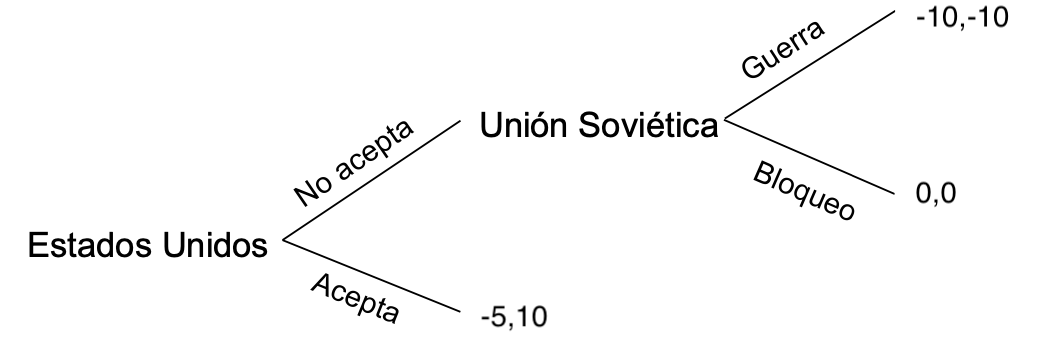
\includegraphics[scale=0.5]{Figuras/juegos secuencia.png}  
\end{center}
Las estrategias serán un plan de acción, en esta caso serían (Acepta, No Acepta y Guerra, No Acepta y Bloqueo).

Para resolver estos juegos uno tiene que seguir un método inductivo, resolver desde el futuro hacia el pasado. ¿Por qué resolver de adelante hacia atrás? Porque si resolvieramos como en juegos simultáneos no estaríamos contando si la amenaza (en este caso una respuesta bélica) es creíble. 

Si plantearamos de manera simultánea encontramos dos EN, uno (el de Acepta y Guerra) en que \textbf{no es secuencialmente racional}, para que ese equilibrio sea posible Estados Unidos tiene que aceptar, sin embargo veremos a continuación por qué si Estados Unidos no acepta la Unión Soviética nunca responderá con una respuesta bélica.

\begin{table}[!htbp]
    \centering
    \caption{Dominio sobre Berlín}
    \setlength{\extrarowheight}{2pt}
    \begin{tabular}{*{4}{c|}}
      \multicolumn{2}{c}{} & \multicolumn{2}{c}{Unión Soviética}\\\cline{3-4}
      \multicolumn{1}{c}{} &  & Guerra & Bloqueo \\\cline{2-4}
      \multirow{2}*{Estados Unidos}  & Acepta & $(\underbar{-5},\underbar{10})$ & $(-5,10)$ \\\cline{2-4}
      & No acepta & $(-10,-10)$ & $(\underbar{0},\underbar{0})$ \\\cline{2-4}
    \end{tabular}
  \end{table}

El juego tiene que ser \textbf{secuencialmente racional} por lo que resolvemos de adelante hacia atrás. El resultado será un equilibrio perfecto en subjuegos (EPS).

Por lo tanto primero se resuelve la decisión de la Unión Soviética, la cual debiese decidir bloquear, y luego evaluar que decidirá Estados Unidos, la cual debiese no aceptar. 

\begin{center}
    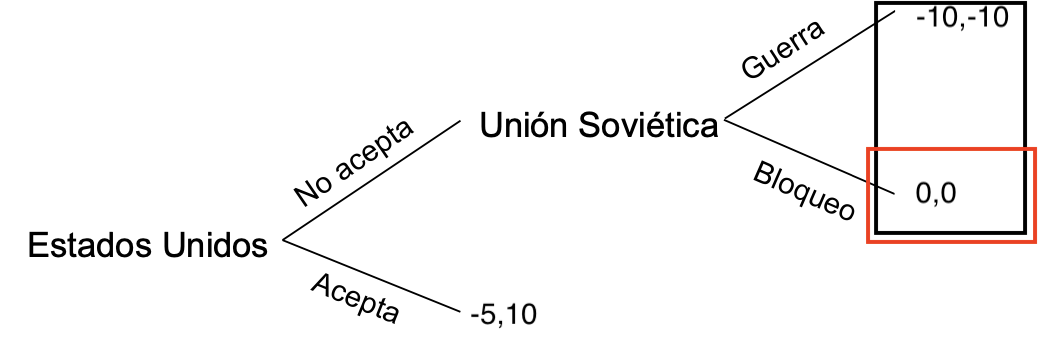
\includegraphics[scale = 0.50]{Figuras/Inducción.png}
\end{center}

\subsubsection*{Relación EN y EPS}

En un juegos secuencial puedes obtener EN que no sean coherentes con las amenazas creíbles. Los EPS siempre son coherentes con la credibilidad de las amenazas. \textbf{Un EN no siempre es un EPS, pero un EPS siempre es un EN}. 

\section{Competencia imperfecta}

\subsection{El factor estratégico}

Los \textbf{oligopolios},\marginnote{\textbf{Oligopolio:} Mercado con un número reducido de firmas las cuales pueden incidir en el precio.}[0cm] también llamados mercados de competencia imperfecta, son un escenario en el cual un número reducido de empresas inciden en cierta medida en el precio de mercado. Es por esto que se le considera un entremedio entre monopolio y competencia perfecta, no eligen libremente pero tampoco son tomadores de precio. 

Todas las firmas tienen cierto poder sobre el precio de mercado, directamente fijando los precios o indirectamente decidiendo las cantidades a producir. Debido a que todas las firmas afectan el precio habrá \textbf{interdependencia monopolística},\marginnote{\textbf{Intedependencia monopolística:} De manera más general llamado interdependencia estratégica. Las empresas toman sus decisiones formando creencias de lo que hará su competencia.}[-1cm] lo cual sugiere que hay un factor estratégico en las competencias olipólicas. Por ejemplo, si una firma fija cierto precio, su rival puede responder con un precio menor para quedarse con una mayor demanda.\footnote{Esto asumiendo que son bienes perfectamente sustitutos (producto homogéneo).} También, si se cree que la firma rival va a producir mucho del bien, a las demás firmas les conviene producir menos para no desplomar el precio de mercado por un exceso de oferta. Es decir, las decisiones de una firma afectan a su competencia y viceversa, ante esto las firmas formarán creencias de lo que hará la competencia para tomar sus propias decisiones. 

\subsubsection*{La estrategia desde la teoría de juegos}

La manera en que entendemos estas interacciones propias de la \textbf{organización industrial}\marginnote{\textbf{Organización industrial:} Área de la teoría de la firma que se enfoca en la estructura e interacciones en los mercados.} es mediante la teoría de juegos. Tal como se mencionaba antes, en la teoría de juegos los jugadores tienen que formar una creencia de lo que hará el otro para reaccionar de la mejor manera. A continuación plantearemos como se verían estos juegos aplicado a los distintos tipos de competencia imperfecta. 

Para esta ocasión solo se abarcarán juegos normales, es decir, los jugadores $i \in 1,2,\ldots,N$ serán racionales y deciden su acción o combinación de acciones $a_i \in A_i$ resultando en un pago $\pi_i(a)$ para cada firma.

Las firmas elegiran $a_i$ de manera de maximizar sus pagos, una estrategia será mejor que otra mientras el pago resultante sea mayor. Dado que los rivales $-i$ escogen una estrategia $a_{-i}$, la firma $i$ tendrá una respuesta óptima $a_i^*$ en que los pagos sean mayores, es decir,\footnote{Dada las características del juego y considerando que los individuos son racionales es esperable que siempre elijan la respuesta óptima $a_i^*$.} 
\begin{equation}
    \pi_i(a_i^*, a_{-i}) \geq \pi_i(a_i, a_{-i}), \forall a_i . \label{eq: mejor respuesta}
\end{equation}
Esto es equivalente a decir que jugando piedra papel o tijera, si mi rival elige tijera la mejor respuesta para el papel es la tijera, mientras que la mejor respuesta para la tijera es la roca. Podremos describir matemáticamente la mejor respuesta de $i$ en función de la estrategia de los demás; $a^*_i(a_{-i})$. A esto se le conoce como \textbf{función de reacción}.\marginnote{\textbf{Función de reacción:} Función que describe la mejor forma de responder ante las decisiones de un competidor.} Cuando todas las firmas elijan su mejor estrategia $a^* \equiv (a_1^*,\ldots,a_N^*)$ no habrán incentivos a cambiar de estrategia, por lo que nos encontraríamos en el Equilibrio de Nash.\footnote{En el caso de piedra papel o tijeras no habría Equilibrio de Nash, suponiendo que todas las opciones tienen las misma probabilidad de ser elegidas.} 

Las firmas seguiran esta manera de pensar para decidir que tienen que hacer al competir con otra firma. En el corto plazo las firmas suelen tomar acciones respecto a la fijación de precios o al nivel de producción, en el largo plazo se podría hablar de entradas a mercado o de inversión en I+D, etc. Veremos a continuación dos modelos que discuten tipos de competencia por precios y cantidades.

\subsection{Competencia a la Bertrand}

\subsubsection{Planteamiento}
Este modelo fue planteado por el matemático \textbf{Joseph Bertrand}\marginnote{\textbf{Joseph Bertrand (1822-1900):} Matemático francés del siglo XIX. Proporcionó aportes a la economía como fue el modelo de Bertrand. Fue crítico del principio de maximización de utilidad.}[0cm] en 1883. Vamos a pensar en un duopolio de firmas $i\in 1,2$ que ofrecen un producto homogéneo compitiendo precios $p_i$. 

Como los productos son homogéneos, es decir son sustitutos perfectos, la firma que ofrezca el menor precio se llevará toda la demanda $Q_i(p_i)$, en caso de ofrecer un mismo precio se reparten la demanda de manera equitativa. Por lo demás, las firmas tendrán un costo marginal $c_i$. 

Para entender como se llega al equilibrio en este mercado primero tenemos que identificar cuales son las mejores respuestas de una firma ante acciones de la otra, es decir la $a^*_i(a_{-i})$. Pensando desde el punto de vista de la firma $1$ podemos considerar 3 casos posibles y sus respectivas respuestas ante acciones de la firma $2$, buscamos definir la función de reacción $p^*_1(p_2)$.

\begin{itemize}
    \item En caso de que la firma $2$ fije un precio $p_2$ mayor al precio monopólico $p_1^M$. La mejor respuesta es fijar el precio monopólico, de esta manera maximizan beneficios mientras absorben toda la demanda.
    \item Si la firma $2$ fija un precio menor al precio monopólico $p_1^M$ y mayor a al costo marginal $c_1$. Para capturar toda la demanda conviene fijar un precio minúsculamente menor al de la competencia, lo cual se denota como $p_1-\epsilon$ siendo $\epsilon$ un número positivo cercano al cero.
    \item La firma $2$ fija un precio igual o menor al costo marginal $c_1$. Para estos casos la mejor respuesta es fijar el costo marginal.
\end{itemize}

El precio $p_1$ que fije la firma $1$ en función de $p_2$ puede ser descrito en esta función y representado en la figura \ref{fig:funciones de reacción Bertrand},
\begin{align*}
    p^*_1(p_2)= \left\{ \begin{array}{lcc} p_1^M & \text{si} &  p_2> p_1^M \\ \\ p_2-\epsilon & \text{si} & p_1^M \geq p_2>c_1 \\ \\ c_1 & \text{si} & c_1 \geq p_2 \end{array} \right.
\end{align*}

\begin{figure}[htb]
    \centering
    \caption{Funciones de reacción de competencia tipo Bertrand con firmas simétricas}
    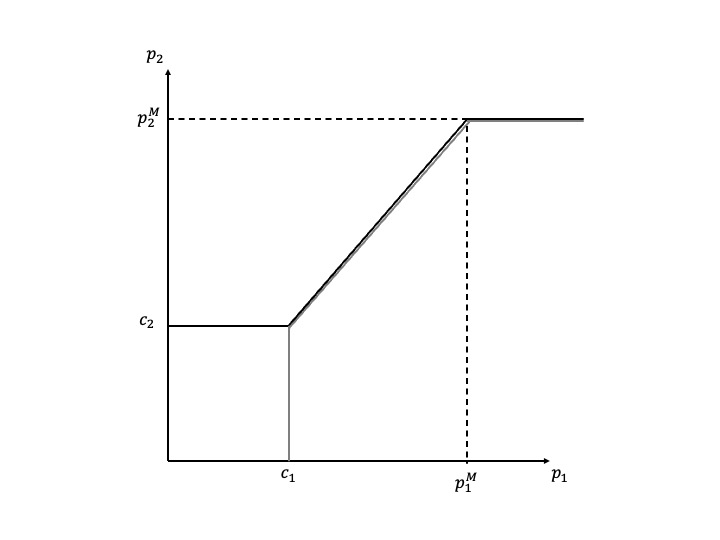
\includegraphics[width=15cm]{Figuras/Función de reacción Bertrand.jpeg}
    \label{fig:funciones de reacción Bertrand}
\end{figure}


\subsubsection{Equilibrios de competencia a la Bertrand}

Un caso útil para describir la dinámica se da cuando las empresas son simétricas, lo cual implica que tienen un mismo costo marginal $c$. La dinámica aquí es que la mejor respuesta ante cualquier precio $p_{-i}^M \geq p_i>c$ será fijar un precio menor, ante lo cual la competencia debería responder con un precio aun menor. De esta manera el precio bajará hasta el punto en que tanto $p_1$ como $p_2$ sean iguales a $c$. 

Este caso es conocido como la \textbf{paradoja de Bertrand}.\marginnote{\textbf{Paradoja de Bertrand:} Durante la competencia de un duopolio con firmas simétricas el equilibrio de Nash se da donde el precio es igual al costo marginal. Es decir, se llega al resultado de competencia perfecta con sólo 2 firmas.}[-3.5cm] Se le da este nombre puesto que el resultado de esta competencia imperfecta con 2 firmas es el mismo que en competencia perfecta ($p=c$). Tal como se ve en la figura \ref{fig:EN Bertrand sim}. 

\begin{figure}[htb]
    \centering
    \caption{Equilibrio de Nash en Bertrand con firmas simétricas}
    \includegraphics[width=15cm]{Figuras/EN Bertrand con firmas simétricas.jpeg}
    \label{fig:EN Bertrand sim}
\end{figure}

El resultado de una competencia en que una firma es más eficiente dista de lo anterior. Cuando una firma tiene un costo marginal menor a su rival podrá absorber toda la demanda fijando un precio ligeramente menor al costo marginal de su competencia. Más precisamente en el caso en que $c_1<c_2$ el equilibrio resulta en $p_1 = c_2 - \varepsilon$. Lo cuál llevaría a la firma menos eficiente a salir del mercado y la firma ganadora obtendría beneficios. Vease \ref{fig:EN Bertrand asim}. 

\begin{figure}[htb]
    \centering
    \caption{Equilibrio de Nash en Bertrand con firmas asimétricas}
    \centering
    \includegraphics[width=15cm]{Figuras/EN Bertrand firmas asimétricas.jpeg}
    \label{fig:EN Bertrand asim}
\end{figure}

\subsection{Competencia a la Cournot}

\subsubsection{Planteamiento}

Otra manera de modelar la competencia entre firmas $i \in 1,2$ es mediante las cantidades de producción de cada una, lo cual se puede extrapolar a mercados con nula diferenciación de producto (Nuevamente nos referimos a productos homogéneos).\footnote{Por ejemplo, no importa la marca del cobre, no hay diferenciación de producto. El mayor predictor del precio asumiendo fija la demanda será la oferta.} El matemático francés \textbf{Antoine Cournot}\marginnote{\textbf{Antoine Cournot (1801-1877):} Filósofo y matemático frances que impulso la economía marginalista. Fue de los primeros quienes empezaron a usar funciones matemáticas para describir relaciones como la oferta y la demanda}[-4.5cm] planteó un modelo de mercado de un bien homogéneo donde la única variable estratégica que manejan las firmas es el nivel de producción.

Presentaremos el modelo dentro de un duopolio en donde cada firma produce una cantidad $q_i$, donde el total producido $Q$ es la suma de las producciones individuales.
\begin{equation}
    Q = \sum_{i=1}^N q_i = q_1 + q_2 + \ldots +q_N
\end{equation}
Asumiremos que las firmas son simétricas (mismo costo marginal) y enfrentan una misma demanda inversa lineal $P(Q) = A - Q$. 

Para resolver el modelo debemos de plantear el problema que enfrenta cada firma. Esto es, maximizar beneficios considerando lo que pueden producir y vender $q_i$ y el beneficio marginal de cada producto $P-c$.
\begin{equation}
    \max_{q_i} \quad \Pi _i = (P-c)q_i \label{eq: maximización}
\end{equation}
Como todas las producciones de distintas empresas están contenidas en \ref{eq: maximización} mediante el precio,\footnote{De la manera $P = A-\sum_{i = 1}^Nq_i$.} al optimizar obtendremos la cantidad que debiera producir la firma para maximizar sus beneficios en función de las decisiones de su competencia. Esto es, la estrategia óptima $q_i^*$ ante la estrategia del rival $q_j$. Resolvemos para la firma $1$.
\begin{align*}
\max_{q_1} \quad \Pi_1 &= (P-c)q_1 = (A-q_1-q_2)q_1 - cq_1 \\
\text{CPO:} \quad \frac{\partial \Pi_1}{\partial q_1} &= A-2q_1 - q_2 -c =0
\end{align*}
Teniendo las condiciones de primer orden solo queda despejar para obtener la función de reacción de la firma $1$ ante la estrategia de la firma $2$.
\begin{equation}
    q^*_1(q_2) = \frac{A-q_2-c}{2} \label{eq: Función de reacción 1}
\end{equation}

La mejor estrategia para $1$ dependerá de la producción de $2$. La producción óptima $q^*_1$ bajará en caso de que el rival produzca más $\Delta^+ q_2$, esto ya que aumentar la producción causaría que el precio caiga más de lo ideal por el exceso de oferta. Es por esto que en competencias a la Cournot la pendiente de la función de reacción será negativa.\footnote{En Bertrand hay pendiente positiva en ciertas partes de la función puesto que un aumento de precio de una firma no llevaba a una reducción del precio de la otra.}

\subsubsection{Equilibrio de competencia a la Cournot} 

Recordemos que las firmas llegarán a un equilibrio de Nash cuando estas respondan su estrategia óptima ante la estrategia óptima de sus competidoras. Dadas las funciones de reacción es trivial encontrar el equilibrio, directamente se reemplaza la función de respuesta $q^*_2(q_1)$ en $q^*_1(q_2)$ o viceversa.

\begin{figure}[htb]
    \centering
    \caption{Equilibrio de Nash en Cournot}
    \centering
    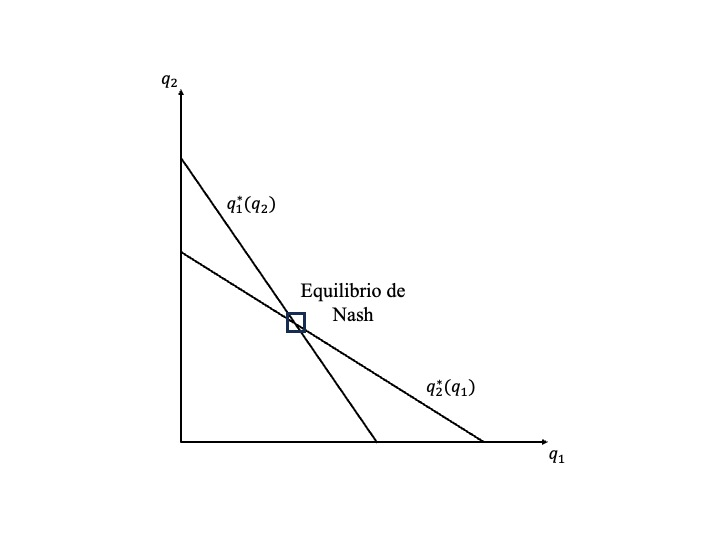
\includegraphics[width=12cm]{Figuras/EN Cournot.jpeg}
    \label{fig:EN Cournot}
\end{figure}

Como en este caso las firmas son simétricas podemos decir que $q_1 = q_2 = q$ y resolver directamente. 
\begin{align}
    q &= \frac{A-q-c}{2} \notag \\
    q &= \frac{A-c}{3} \label{eq: producción individual}
\end{align}
Según \ref{eq: producción individual} tendremos la producción individual de las dos firmas.

El precio se determinará por el total de oferta en el mercado, es decir, la producción de cada una de las firmas $Q = 2q$. 
\begin{align}
    P &= A-2 \cdot \left( \frac{A-c}{3} \right) \notag \\
    P &= \frac{A-2c}{3}
\end{align}
Por último podemos determinar los beneficios de cada firma reemplazando los valores en \ref{eq: maximización}
\begin{align}
\Pi_i &= \left(\frac{A-2c}{3}-c \right) \frac{A-c}{3} \notag \\ 
\Pi_i &= \frac{(A-c)^2}{9}
\end{align}

Este ejemplo de equilibrio es con firmas simétricas, en caso de haber una firma más eficiente a esta le convendría producir más. Graficamente la empresa más eficiente debiera tener una función de reacción más desplazada hacia la derecha. 

\subsubsection*{Caso para $n$ firmas}
Como ejercicio se recomienda hacer este mismo procedimiento para $n$ firmas en el mercado. Una vez hecho se recomienda analizar los efectos marginales de aumentos o reducciones en $n$ y el caso en que $n$ tiende a infinito.


\section*{Recapitulación y observaciones}

En los dos tipos de competencia las firmas forman creencias de lo que hará la competencia para poder maximizar beneficios. En el caso de Bertrand presentado la solución es directa y no se requiere de plantear el problema de maximización de beneficios. 

Se puede notar mirando los beneficios en cada caso, que competir a la Bertrand es mucho más competitivo que a la Cournot. Una empresa más eficiente que su competencia en Cournot podrá vender más, en Bertrand se quedará con todo el mercado. 

En los casos presentados se supone implícitamente que las empresas tienen capacidad de servir a todo el mercado que quieran. Este supuesto no es realista y se puede levantar dando pasos a otras conclusiones pero que no se desvían mucho de lo ya visto. Se puede encontrar más detalle en el anexo. 

\subsection{Competencia a la Stackelberg}

Este modelo fue propuesto por el economista alemán \textbf{Heinrich von Stackelberg}.\marginnote{\textbf{Heinrich von Stackelberg (1905-1946)}: Economista alemán de ascendencia argentina nacido en Rusia, arrepentido miembro del Partido Nazi y sargento de la SS, falleció en España. Aportó a la teoría de juegos.}[0cm] Ya habiendo comprendido el modelo Cournot no es complejo entender el modelo Stackelberg.\footnote{Competencia a la Stackelberg es una tipo de competencia a la Cournot.} El \textit{twist} con respecto al modelo anterior se encuentra en que las firmas jugarán por turnos, inevitablemente la primera a jugar tiene la ventaja. 

Supongamos que la firma $1$ es la líder pues juega primero, mientras que la firma $2$ es la seguidora. La firma líder decidirá en el $t = 1$ la cantidad $q_1$ que producirá y en $t=2$ la firma seguidora decidirá su producción $q_2$ en función de $q_1$.

Este tipo de juegos se tienen que resolver por inducción. Si miramos el problema desde el final hasta el inicio primero se maximizan los beneficios de la firma $2$, la cual en $t = 2$ ya sabrá qué produjo la firma $1$, de lo cual obtendremos $q_2^*(q_1)$. La firma líder tendrá que maximizar en $t=1$ sujeto a lo que hará la seguidora en $t=2$. El problema de la firma $1$ se plantea de la siguiente manera,
\begin{align*}
    \max_{q_1} \quad &\Pi_1 = (P(Q)-c)q_1 \\
    \text{s.a}\quad &q_2=q_2^*(q_1)
\end{align*}
Suponiendo una demanda lineal y que las firmas son simétricas podemos considerar (\ref{eq: Función de reacción 1}) como la función de reacción para la firma seguidora. Reemplazamos la restricción en la expresión a maximizar y reescribimos el problema como,
\begin{align*}
    \max_{q_1} \quad &\Pi_1 = \left(A-q_1-c- \left(\frac{A-q_1-c}{2} \right) \right)q_1 \\ & \Pi_1 = \left( \frac{A-q_1-c}{2}   \right)q_1 \\
    \text{CPO:} \quad & \frac{\partial \Pi_1}{\partial q_1} =   \frac{A-c}{2} -q_1 = 0 \\
    & q_1 = \frac{A-c}{2}
\end{align*}
Reemplazando $q_1$ en $q_2^*(q_1)$ obtendremos la producción de la firma seguidora. 

La producción de la firma líder aumenta por sobre el caso de Cournot con turnos simultáneos. La firma líder tiene más espacio para aumentar la producción para aumentar ventas, mientras que la seguidora tendrá que adaptarse produciendo menos para que el precio no baje demasiado.


\section{Acuerdos colusivos}

Como se puede notar en el problema de la firma, cada empresa maximiza los beneficios propios y no los conjuntos, lo cual es un factor en el nivel competitivo de las firmas y el poder de mercado que ostenten. Sin embargo, la competencia no es buena para las firmas, al haber más firmas lo esperable es que el precio vaya convergiendo al costo marginal, lo cual muestra como van perdiendo poder de mercado. La colusión es una manera en que las firmas se compromoten a colaborar para aumentar las utilidades personales. 

En la realidad se ven distintos tipos de colusiones las cuales dependiendo el producto tomarán diferentes formas; Aumento de precios, reducción de oferta, restricciones territoriales y mecanismos de castigo. Es útil para las instituciones fiscalizadores estudiar y comprender los factores que podrían indicar una colusión o que faciliten un acuerdo colusivo. 

La teoría de juegos nos ayuda a modelar las decisiones de las firmas mediante \textbf{juegos iterativos}.\marginnote{\textbf{Juegos iterativos:} Juegos en los cuales hay más de un período/turno en que se juega. Pueden ser finitos e infinitos.}[-3cm] Sin embargo hay que considerar un punto muy importante, en caso de períodos finitos no es posible el \textbf{equilibrio perfecto en subjuegos}\marginnote{\textbf{Equilibrio perfecto en subjuegos:} En los juegos dinámicos de información perfecta habrá un equilibrio perfecto en subjuegos cuando se de un equilibrio por inducción en donde todas las decisiones sean creíbles.} colusivo, sólo será posible en iteraciones infinitos lo cual se explicará más adelante.

En este tipo de acuerdos habrá un incentivo a traicionar, es decir, desviarse del acuerdo para conseguir incluso mayores utilidades de las que conseguirían coludiéndose. En caso de que esto ocurra las demás empresas seguirán una \textbf{estrategia gatillo}, provocando que se acabe la fase de colaboración y empiece la fase de castigo. El castigo es empezar a competir normalmente por el resto del juego, ya sea a la Bertrand, Cournot, etc.

En los casos finitos de $T$ períodos de tiempo nunca habrá incentivos para cooperar en el último período. Como no hay un mañana $T+1$ no habría fase de cástigo por desviarse en $T$, todos preferiran traicionarse el uno al otro. En $T$ nadie coopera lo cual induce a que nadie coopere en $T-1$, el resultado es que nadie coopera en ninguno de los períodos. Nunca hay colusión con períodos finitos, mientras que existen equilibrios colusivos en $T$ infinitos cumpliendose ciertas condiciones. Una empresa se coludirá perpetuamente en caso de que los beneficios de coludirse sean mayores a los de no hacerlo. 

\subsection*{Planteamiento}

Las firmas al coludirse estarán ponderando si es que los beneficios de traicionar en el corto plazo compensarán los beneficios de mantenerse coludidos en el largo plazo. Si una firma se desvía quiere decir que en ese turno gana los beneficios extraordinarios $\pi^D$, los cuales suelen ser los beneficios monopólicos $\pi^M$, durante los siguientes turnos por estrategia gatillo todos empiezan a competir obteniendo en este caso $\pi^G$.\footnote{$\pi^G$ va a depender del las condiciones del mercado, demanda, competidores, tipo de competencia; Cournot, Bertrand, Stackelberg, etc.}

Además se tiene que considerar que los beneficios de períodos más lejanos al presente tendrán menos peso para las decisiones de las firmas. De manera similar al modelo de consumo intertemporal vamos a ponderar los períodos futuros por un descuento $0 \leq \delta < 1$ para todos los períodos $t \in 0,1,2,\ldots,T$.

\subsubsection*{Condición de colusión para Bertrand}

Vamos a ver un caso específico para introducirnos en la dinámica. En el caso de un duopolio Bertrand con firmas simétricas ($\pi^G=0$ y $\pi^D = \pi^M$) podemos describir los beneficios de desviarse $V^D$ en el período $t=0$ como,\footnote{El factor $\frac{\delta}{1-\delta}$ viene de la suma geométrica.}
\begin{equation}
    V^D = \delta^0 \pi^M + \delta \pi^G + \delta^2 \pi^G+ \ldots + \delta^T \pi^G= \pi^M + \frac{\delta}{1-\delta} \pi^G = \pi^M \label{eq: Desvío del acuerdo competencia a la bertrand}
\end{equation}
\ref{eq: Desvío del acuerdo competencia a la bertrand} denota las utilidades de desviarse y obtener beneficios monopólicos en el primer turno y luego competir a la Bertrand obteniendo cero beneficios. En caso de seguir la colusión calculamos $V^C$ como el reparto de las utilidades monopólicas $\frac{\pi^M}{N}$. 
\begin{equation}
    V^C = \delta^0 \frac{\pi^M}{2} + \delta ^1 \frac{\pi^M}{2} + \delta ^2 \frac{\pi^M}{2} +\ldots + \delta^T \frac{\pi^M}{2} = \frac{\pi^M}{2} + \frac{\delta}{1-\delta} \frac{\pi^M}{2}
\end{equation}
La colusión se dará cuando para cada empresa se cumpla que, 
\begin{equation}
    V^C \geq V^D
\end{equation}
Para evaluar si esto ocurre tendremos que fijarnos que la tasa de descuento $\delta$ cumpla ciertas condiciones,
\begin{align*}
    V^C \geq V^D \Longleftrightarrow \frac{\pi^M}{2} + \frac{\delta}{1-\delta} \frac{\pi^M}{2} \geq \pi^M \\
    \text{Despejando $\delta$ obtenemos la condición} \quad \delta \geq \frac{1}{2}
\end{align*}

Es decir, mientras se cumpla que $\delta \geq \frac{1}{2}$ el acuerdo colusivo se va a dar en todos los períodos. La interpretación es que si las firmas tienen un nivel de paciencia suficientemente alto para valorar los beneficios de coludirse a largo plazo, preferiran mantener el acuerdo antes de los beneficios de corto plazo del desvío. 

\subsubsection*{Colusiones, caso general}

Una fórmula general de expresar lo anterior es la siguiente,
\begin{equation}
    \frac{\delta }{1-\delta} (\pi ^C - \pi^{G}) \geq \pi ^D- \pi^C \label{eq: Condición de colusión generalizada}
\end{equation}

Donde $\pi^C$ serán los beneficios que recibe la empresa al coludirse con las demás,\footnote{Nótese que es diferente a $\pi^M$ puesto que se tienen que repartir entre las firmas coludidas.} $\pi^D$ son los beneficios del turno al desviarse y $\pi^G$ serán los beneficios donde por estrategia gatillo todas las firmas empiecen a competir. \ref{eq: Condición de colusión generalizada} se interpreta como que los beneficios a largo plazo deben ser más valorados que los beneficios a corto plazo. 

De \ref{eq: Condición de colusión generalizada} también podemos despejar el descuento $\delta$. De esta manera conseguiremos el $\delta$ mínimo para asegurar que la colusión se cumpla.
\begin{equation}
    \delta \geq \frac{\pi^D - \pi ^C}{\pi^D- \pi^G} \label{eq: Condición que tiene un nombre del que no me acuerdo ;(}
\end{equation}

\subsection{Factores que facilitan o dificultan la colusión}

Hay distintos factores que pueden facilitar la colusión, el factor de descuento es uno de ellos. Derivaremos los siguientes factores:
\begin{itemize}
    \item A mayor cantidad de firmas más díficil es mantener un equilibrio colusivo.
    \item Ante una fase de castigo más severa es sea más fácil mantener la colusión.
    \item En caso de asimetría en las firmas, habrá quienes sean más propensas o menos propensas a mantener el trato.
\end{itemize}

\subsubsection*{Cantidad de firmas y acuerdos colusivos}

Para un número de $N$ firmas iguales compitiendo a la Cournot las utilidades de coludirse bajaran con la cantidad de firmas, $\pi^C = \frac{\pi^M}{N}$. Si en un turno una firma se desvía ganan $\pi^M$, para simplificar diremos que en la fase de castigo $\pi^G = 0$.

Citando \ref{eq: Condición que tiene un nombre del que no me acuerdo ;(} y reemplazando los beneficios para este caso obtenemos el descuento mínimo necesario para que la colusión sea posible $\bar{\delta}$. 
\begin{align*}
    \delta \geq \frac{\pi^M - \frac{\pi^M}{N}}{\pi ^M - 0} \Longleftrightarrow &\bar{\delta} = 1 - \frac{1}{N} \\
    & \frac{\partial \bar{\delta}}{\partial N} > 0
\end{align*}

A mayor cantidad de firmas es más difícil que las empresas se coludan pues requieren ponderar en mayor medida los beneficios a largo plazo del acuerdo. Es por esto que las instituciones fiscalizadores ponen especial atención en mercados con pocas firmas. 

\subsubsection*{Fases de castigo y acuerdos colusivos}

Es intuitivo pensar que si el castigo es mayor es más fácil alcanzar un acuerdo colaborativo. Anteriormente se mencionó como Bertrand es un tipo de competencia más fuerte que Cournot, lo cual conlleva que sea más fácil llegar a acuerdos colusivos en Bertrand que en Cournot. Esto se puede ver directamente en la expresión \ref{eq: Condición que tiene un nombre del que no me acuerdo ;(}, competir a la Cournot suele resultar en que $\pi^G$ sea mayor que en Bertrand. 
\begin{align*}
    \frac{\partial \bar{\delta}}{\partial \pi^G} > 0
\end{align*}

Al haber menos castigo es necesaria mayor paciencia para mantener el acuerdo. 

\subsubsection*{Asimetría en las firmas y acuerdos colusivos}

Un punto muy relacionado a lo anterior es el tema de acuerdos colusivo entre firmas asimétricas. En un acuerdo la firma más eficiente tendrá una suerte de dominancia por sobre la otra puesto que en caso de competir la más eficiente saldrá mejor parada. Es por lo anterior que las firmas más eficientes requerirán de mayor paciencia mínima $\bar{\delta}$ para mantener el acuerdo. 

\begin{appendices}
    \chapter{Anexo}

\section{Cournot con restricciones de capacidad}

De forma complementaria se puede levantar el supuesto de que una sola empresa podría servir a todo el mercado si así lo quisiera. Algo más parecido a la realidad es que una sola firma no puede servir a todo el mercado aunque así lo quisiera. La capacidad de una firma puede denotarse como $K$. Frente a una demanda inversa lineal $P(Q) = A-Q$ y considerando dos firmas idénticas de $c=0$ tendremos restricciones activas de capacidad en caso de que $K \leq A$. 

En caso de que compitan la pregunta es qué parte de la curva de demanda sirve cada firma. Se puede asumir racionamiento eficiente, en caso de haber dos precios distintos el más barato será el primero en venderse a los que están más dispuestos a pagar. Una vez vendida toda la capacidad de la firma más barata la otra firma se queda con el sobrante.
\end{appendices}

\end{document}